
\documentclass[ms.tex]{subfiles}
\begin{document}

\section{Galactic Properties}
\label{sec:galprops}

\begin{figure*}
\centering
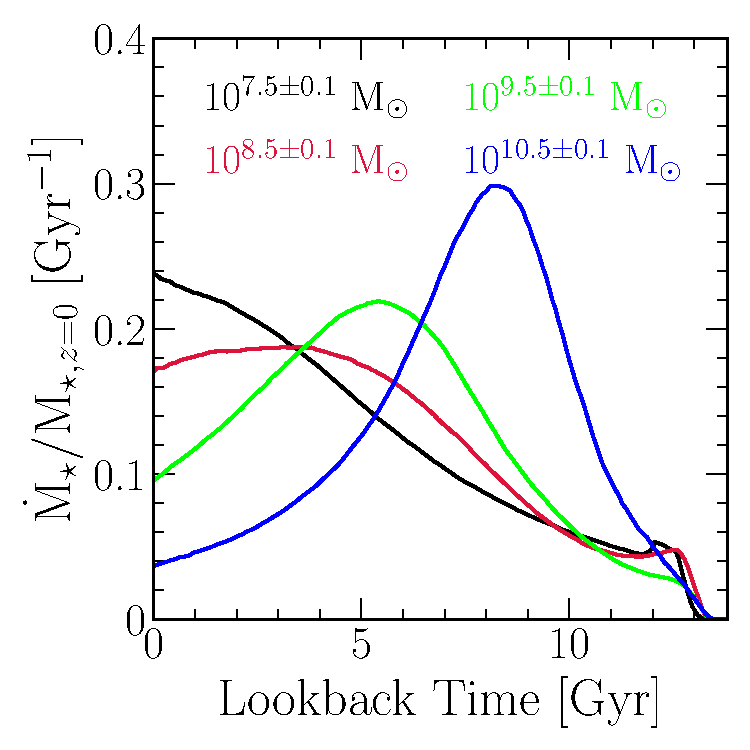
\includegraphics[scale = 0.43]{umachine_sfhs.pdf}
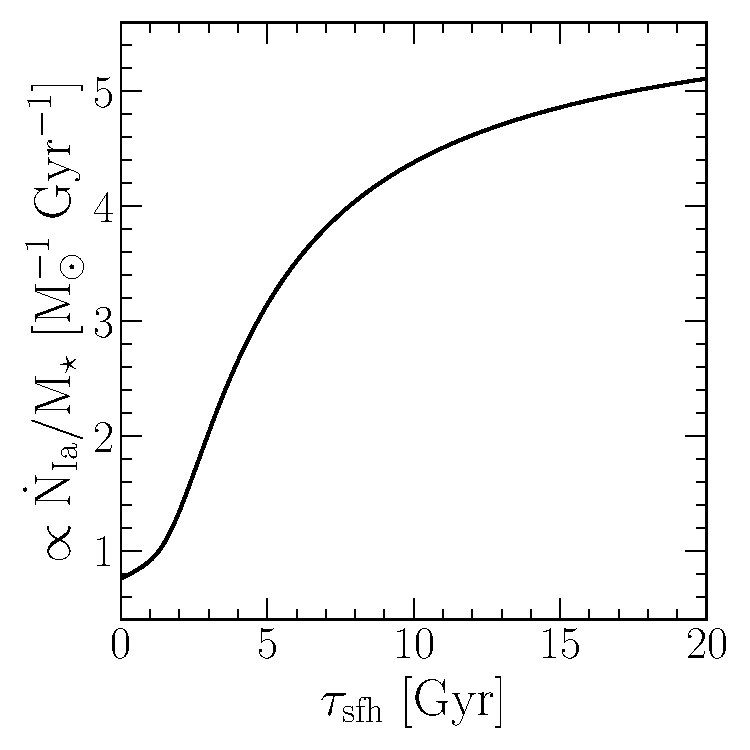
\includegraphics[scale = 0.42]{iarate_vs_tausfh.pdf}
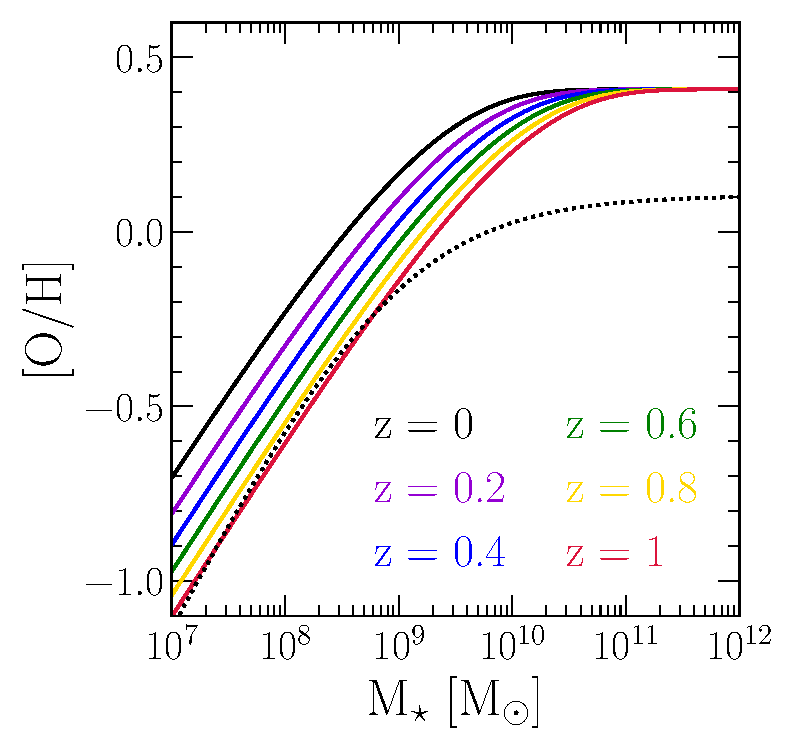
\includegraphics[scale = 0.42]{mzr.pdf}
\caption{Star formation histories.}
\label{fig:sfhs}
\end{figure*}

% \subsection{Star Formation Histories}
% \label{sec:galprops:sfhs}

\begin{itemize}

	\item We begin by examining how the mean galactic SFH varies with
	present-day stellar mass as predicted by the~\um~SAM of galaxy formation
	\citep{Behroozi2019}.
	Using dark matter halo properties supplied by the~\textit{Bolshoi-Planck}
	and~\textit{Multi-Dark Planck 2} dark matter only simulations
	\citep{Klypin2016, RodriguezPuebla2016},~\um~follows a conventional
	SAM framework (see, e.g., the review in~\citealp{Somerville2015a}) by
	parametrizing the SFRs of galaxies as a function of lookback time, the
	assembly history of the halo, and the depth of the halo's potential well.
	Like other SAMs that have come before it,~\um~successfully reproduces a
	broad range of well-constrained observables, including stellar mass
	functions, cosmic SFRs, specific SFRs, quenched fractions, UV luminosity
	functions, and more.
	While previous SAMs have used the extended Press-Schechter formalism
	\citep{Press1974, Bond1991} to generate halo merger trees and push the
	lower stellar mass limit of their model down to
	$M_\star \approx 10^7~\msun$~\citep*[e.g.][]{Somerville2015b}, an advantage
	of~\um~is that the high mass resolution of the~\textit{Bolshoi-Planck} and
	\textit{Multi-Dark Planck 2} simulations allows merger trees down to
	$M_\star = 10^{7.2}~\msun$ to be obtained directly from the simulations.
	Dwarf galaxies in this regime are of particular interest to this
	investigation because the~\citet{Brown2019} results on the scaling of the
	specific SN Ia rate with stellar mass reach as low as~$\sim10^7~\msun$ in
	their volume-limited sample and~$\sim10^6~\msun$ in their full sample.

	\item In the left panel of Fig.~\ref{fig:sfhs}, we plot the average SFH as
	a function of lookback time in four narrow bins in observed stellar mass
	taken from~\um.
	In the interest of relating these predictions to data from ASAS-SN, an
	untargeted survey, we take the full galaxy sample from~\um, including both
	star forming and quenched galaxies as well as both centrals and satellites,
	though central galaxies are the dominant population across the full stellar
	mass range.
	In general, low stellar mass galaxies have more extended SFHs than their
	higher mass counterparts.
	This effect is sufficiently strong such that around
	$M_\star \approx 10^{7.5} \msun$, the fastest SFR typically occurs near the
	present day.
	Unless the SN Ia DTD depends on the present-day stellar mass of a galaxy
	in some highly specific manner, this should impact the characteristic SN Ia
	rate as a function of stellar mass.

	\item Although the details of the SN Ia DTD are a topic of active inquiry
	\citep[e.g.][]{Greggio2005, Strolger2020, Freundlich2021}, comparisons of
	the cosmic SFH~\citep[e.g.][]{Madau2014, Madau2017} with the volumetric SN
	Ia rate as a function of redshift suggest that the cosmic DTD is broadly
	consistent with a~$\tau^{-1}$ power-law (\citealp*{Maoz2012a, Maoz2012b,
	Graur2013};~\citealp{Graur2014}).
	A DTD of approximately this form is also expected under the
	double-degenerate scenario given population synthesis models of binary
	white dwarfs and the loss of angular momentum due to graviational wave
	emission (e.g.~\citealp{Mennekens2010};~\citealp*{Maoz2014}).
	We therefore adopt this parametrization in this paper, though we have
	reconducted our analysis using an exponential DTD with a timescale of
	$\tau_\text{Ia} = 1.5$ Gyr and found similar results.
	% This single power-law is also a common choice in galactic chemical evolution
	% (GCE) models~\citep[e.g.][]{Andrews2017, Johnson2021}, though other simple
	% parametrizations such as an exponential~\citep[e.g.][]{Chen2022} are also
	% common.

	\item In principle, the minimum delay~$t_\text{D}$ of the DTD could be as
	short as~$\sim$40 Myr if WDs are produced by~$\lesssim$8~\msun~stars
	\citep*[e.g.][]{Hurley2000}, and perhaps even shorter at low metallicity if
	the total metal content of a star significantly impacts its lifetime as in,
	e.g.,~\citet{Kodama1997} and~\citet{Vincenzo2016}.
	However, if SNe Ia require some additional time following WD formation, the
	minimum delay will be longer.
	Since we are interested in demonstrating the first-order effects of
	variations in SFHs on specific SN Ia rates, we assume a value of
	$t_\text{D} = 100$ Myr.
	We have also reproduced the results of this paper with both
	$t_\text{D} = 40$ Myr and~$t_\text{D} = 150$ Myr and found similar results
	in both cases.

	\item For an SFH~$\dot{M}_\star$ and DTD~$R_\text{Ia}$ as functions of
	lookback time~$\tau$, the specific SN Ia rate can be expressed as
	\begin{equation}
	\frac{\dot{N}_\text{Ia}}{M_\star} =
	\ddfrac{
		\int_0^{T - t_\text{D}} \dot{M}_\star(\tau) R_\text{Ia}(\tau) d\tau
	}{
		(1 - f_\text{loss})\int_0^T \dot{M}_\star(\tau) d\tau
	},
	\label{eq:specia}
	\end{equation}
	where~$t = T - \tau$ is the time since the onset of star formation,~$T$
	is the same quantity at the present day, and~$f_\text{loss}$ is a
	corrective term to account for mass loss as stellar populations age.
	While the normalization of the SFH cancels, we omit the normalization of
	the DTD from equation~\refp{eq:specia} because we are not interested in the
	absolute SN Ia rate in the present paper -- only the relative scaling as a
	function of galaxy stellar mass.
	In detail,~$f_\text{loss}$ varies with the age of a stellar population.
	However, the material that is eventually returned to the ISM is dominated
	by high mass stars with short lifetimes, while the loss rate drops quickly
	due to the long lifetimes of their lower mass counterparts.
	It is therefore accurate to first-order to assume that stellar populations
	of all ages have returned~$f_\text{loss} \approx 40$\% of their initial
	mass back to the ISM (appropriate for a~\citealt{Kroupa2001} IMF;
	$f_\text{loss} = 20$\% for a \citealt{Salpeter1955} IMF; see also the
	discussion in~\S\S~2.2 and 3.7 in~\citealt*{Weinberg2017} demonstrating
	that the age-dependence of~$f_\text{loss}$ is a small correction in
	one-zone galactic chemical evolution models).

	% Because the denominator of this equation represents the present day stellar
	% mass, it should in detail be divided by~$1 - f_\text{loss}(\tau)$,
	% a corrective term to account for mass loss as stellar populations age and
	% return their envelopes to the interstellar medium (ISM).
	% To first order, however, this correction can be reasonably approximated as
	% if~$f_\text{loss} \approx 40$\% of a stellar population's initial mass is
	% immediately returned to the ISM.
	% This arises because relative to a whole stellar population, the mass that
	% is eventually returned to the ISM is dominated by high mass stars with
	% short lifetimes (see Fig. 7 and associated discussion in~\S~3.7 of
	% \citealt*{Weinberg2017};~$f_\text{loss} \approx 40$\% is appropriate for a
	% \citealt{Kroupa2001} IMF).
	% This term then becomes another constant of proportionality which can safely
	% be neglected in the interest of investigating relative SN rates.

	\item To illustrate qualitatively how the specific SN Ia rate scales with
	how prompt or extended the SFH is, we consider the simple example of a
	linear-exponential SFH~$\dot{M}_\star \propto te^{-t / \tau_\text{sfh}}$.
	The middle panel of Fig.~\ref{fig:sfhs} shows equation~\refp{eq:specia}
	as a function of the e-folding timescale~$\tau_\text{sfh}$ assuming
	$T = 13.2$ Gyr in all cases.
	The specific SN Ia rate is lowest in the case of a single episode of star
	formation (i.e.~$\tau_\text{sfh} = 0$) and rises steeply until
	$\tau_\text{sfh} \approx 10$ Gyr.
	The rate begins to flatten for yet longer~$\tau_\text{sfh}$ because the
	galaxy approaches the limit in which the SFH is constant (i.e.
	$\tau_\text{sfh} \gg T$).
	Although a~$\tau^{-1}$ DTD is significantly extended, it is not so extended
	such that galaxies with sharply declining SFHs can sustain high SN Ia rates
	from the earliest epochs of star formation.
	A higher specific SN Ia rate as observed in dwarf galaxies is therefore a
	natural consequence of their more extended SFHs, though we demonstrate
	below that this accounts for only a factor of~$\sim$2 between~$10^7$
	and~$10^{10}$~\msun.

	\item Dwarf galaxies not only have more extended SFHs, but they are also
	known empirically to have a lower metal content~\citep{Tremonti2004}.
	In the right panel of Fig.~\ref{fig:sfhs}, we plot this well known
	``mass-metallicity relation'' (MZR) at a selection of redshifts as
	parametrized by~\citet[][see their equation 5]{Zahid2014}.\footnote{
		We have transformed from their~$\log_{10}$(O/H) measurements to the
		logarithmic abundance relative to the sun according to [O/H]~$\equiv
		\log_{10}(N_\text{O} / N_\text{H}) - \log_{10}(N_{\text{O},\odot} /
		N_{\text{H},\odot})$ assuming the solar oxygen abundance derived
		by~\citet{Asplund2009}.
	}
	At low metallicities, there are multiple effects which could increase the
	SN Ia rate.
	At fixed initial mass, low metallicity stars leave behind more massive WDs
	\citep{Umeda1999, Willson2000, Marigo2007, Meng2008, Zhao2012, Kalirai2014}.
	This arises because a low metal content plasma has a lower Rosseland mean
	opacity, leading to weaker winds and lower mass loss rates, enhancing the
	growth of the core during the AGB phase.
	This could make it easier for a WD to reach the Chandrasekhar mass and
	explode (see discussion in~\citealt{Kistler2013}).
	Additionally, the stellar close binary fraction is known to increase from
	$\sim20$\% near solar metallicity to~$\sim40$\% at~$\sim$one fourth solar
	metallicity (the characteristic abundance of a~$10^{7.2}~\msun$ galaxy
	to~\citealt{Zahid2014}).
	Due to their low metallicities, dwarf galaxies should therefore have more
	massive WDs and a higher close binary fraction.
	They should consequently have more potential SN Ia progenitors per unit
	mass of star formation than larger galaxies.

	\item Although we are interested in five decades of stellar mass in this
	paper ($10^7 - 10^{12}~\msun$),~\citet{Zahid2014} present measurements only
	for the~$\sim10^9 - 10^{11}~\msun$ range.
	We have therefore duplicated our results at~$z = 0$ using the parametric
	form of~\citet{Andrews2013}, but we retain the~\citet{Zahid2014} formalism
	in~\S\S~\ref{sec:predictions} and~\ref{sec:diagnostics} below because we
	also compute predicted SN Ia rates out to redshift~$z = 1$.
	By using stacked spectra from the seventh data release of the Sloan Digital
	Sky Survey~\citep{Abazajian2009}, they are able to increase the
	signal-to-noise of the weak [OII] and [OIII] auroral lines at 7320, 7330
	and 4363~\AA~to obtain direct measurements of the electron temperatures
	and abundances in bins of stellar mass extending as low as
	$\sim10^{7.4}~\msun$.
	We compare the two MZRs in the right panel of Fig.~\ref{fig:sfhs}.
	The~\citet{Andrews2013} parametrization has a lower plateau, but otherwise
	a similar slope and turnover mass.
	We find similar results in~\S~\ref{sec:predictions} below using both
	parametrizations because, following~\citet{Brown2019} and
	\citet{Gandhi2022}, we quantify the specific SN Ia rate as a function of
	mass normalized to 1 at~$10^{10}~\msun$.
	Therefore, the slope of the MZR has the most impact on our results because
	this impacts the characteristic metallicities of low mass galaxies relative
	to their higher mass counterparts, and the normalization of the MZR has no
	impact.
	Although neither~\citet{Andrews2013} nor~\citet{Zahid2014} measure the MZR
	above~$10^{11}~\msun$, both suggest that these galaxies should be on the
	plateau anyway.

\end{itemize}

% \subsection{The Mass-Metallicity Relation}
% \label{sec:galprops:mzr}

\end{document}

